\documentclass[a4paper]{article}

% enumerate
\renewcommand{\theenumi}{\alph{enumi}}
\renewcommand{\labelenumi}{\theenumi)}

% itemize
\renewcommand{\labelitemi}{}
\renewcommand{\labelitemii}{$\Rightarrow$}

% argmax
\newcommand{\argmax}[1]{\underset{#1}{\operatorname{arg}\,\operatorname{max}}\;}

\usepackage{amsmath}
\usepackage{amsthm}
\usepackage{mathtools}
\usepackage{wasysym}
\usepackage{bera}
\usepackage{tikz}
\usepackage{multicol}
\usetikzlibrary{calc, shapes.geometric}

\title{Uebung 10}
\author{Shinho Kang\\Baldomero Valdez\\Omar Guti\'errez}
\date{\today}

\newcommand{\mn}[2]{%
   \tikz [remember picture, baseline = (#1.base)]
      \node [inner sep = 0pt, outer sep = 2mm] (#1)
         {$\displaystyle#2$};
}

% no indentation
\setlength{\parindent}{0cm}

\setlength{\jot}{25pt}
\pagestyle{empty}

\tikzstyle{deletion}=[shape=circle,draw=black]
\tikzstyle{square}=[shape=rectangle,draw=black]
\tikzstyle{match}=[shape=rectangle,draw=black]
\tikzstyle{l}=[draw,-latex]

\begin{document}

\maketitle

\begin{multicols}{2}[
\textbf{Exercise 1} Derive the consensus sequence and define match states for a
profile HMM accordingly, only columns with >50\% nucleotides are modeled.
(\_/3)
]

Consensus sequence:

\begin{tabular}{ l l l l l l}
G & C & - & C & T & C \\
G & C & T & - & T & C \\
- & C & - & C & - & A \\
G & - & - & - & T & C \\
A & C & - & C & T & - \\ \hline
\textbf{G} & \textbf{C} & \textbf{-} & \textbf{C} & \textbf{T} & \textbf{C}
\end{tabular}

State annotation:

\begin{tabular}{ l l l l l l}
M & M & D & M & M & M \\
M & M & I & D & M & M \\
D & M & D & M & D & M \\
M & D & D & D & M & M \\
M & M & D & M & M & D \\ \hline
\textbf{0} & \textbf{1} & \textbf{.} & \textbf{2} & \textbf{3} & \textbf{4}
\end{tabular}

\end{multicols}

\begin{figure}[h]
\begin{center}
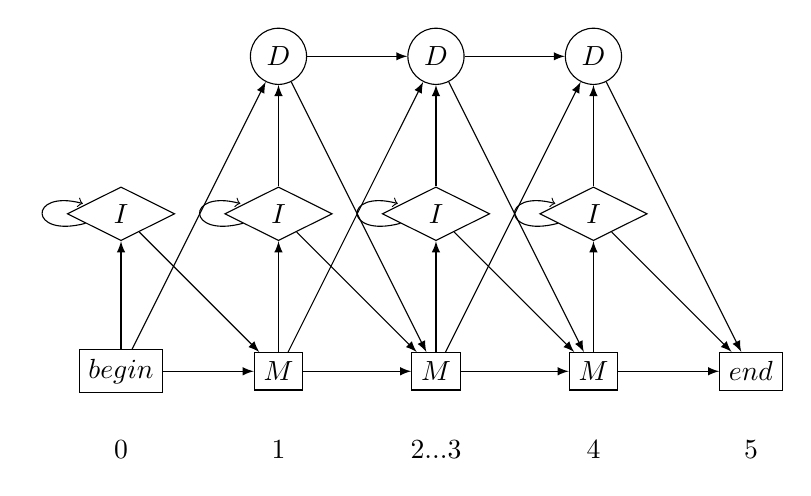
\begin{tikzpicture}[]

% deletion
\node[deletion] (d1) at (2,2) {$D$};
\node[deletion] (d2) at (4,2) {$D$};
\node[deletion] (d3) at (6,2) {$D$};

% insertion
\node[draw, diamond, aspect=2] (i0) at (0,0) {$I$}
edge [loop left] ();
\node[draw, diamond, aspect=2] (i1) at (2,0) {$I$}
edge [loop left] ();
\node[draw, diamond, aspect=2] (i2) at (4,0) {$I$}
edge [loop left] ();
\node[draw, diamond, aspect=2] (i3) at (6,0) {$I$}
edge [loop left] ();

% match
\node[square] (begin) at (0,-2) {$begin$};
\node[match] (m1) at (2,-2) {$M$};
\node[match] (m2) at (4,-2) {$M$};
\node[match] (m3) at (6,-2) {$M$};
\node[square] (end) at (8,-2) {$end$};

% labels
\node[label] (l1) at (0,-3) {$0$};
\node[label] (l2) at (2,-3) {$1$};
\node[label] (l3) at (4,-3) {$2...3$};
\node[label] (l4) at (6,-3) {$4$};
\node[label] (l5) at (8,-3) {$5$};

%paths
\path [l] (d1) -- (d2);
\path [l] (d2) -- (d3);

\path [l] (i0) -- (m1);
\path [l] (i1) -- (m2);
\path [l] (i2) -- (m3);
\path [l] (i3) -- (end);

\path [l] (d1) -- (m2);
\path [l] (d2) -- (m3);
\path [l] (d3) -- (end);

\path [l] (begin) -- (m1);
\path [l] (m1) -- (m2);
\path [l] (m2) -- (m3);
\path [l] (m3) -- (end);

\path [l] (begin) -- (i0);
\path [l] (m1) -- (i1);
\path [l] (m2) -- (i2);
\path [l] (m3) -- (i3);

\path [l] (begin) -- (d1);
\path [l] (m1) -- (d2);
\path [l] (m2) -- (d3);

\path [l] (i1) -- (d1);
\path [l] (i2) -- (d2);
\path [l] (i3) -- (d3);

\end{tikzpicture}
\end{center}
\caption{Profile HMM}
\end{figure}


%$$\hat{b}_{za} = \dfrac{B_{za}}{\sum\limits_{e \in \sum} B_{ze}} $$
%$$\hat{a}_{kl} = \dfrac{A_{kl}}{\sum\limits_{r \in Q} A_{kr}} $$

\end{document}
